\chapter{Workflow}
\label{chap:workflow}

\section{Overview of Analog IC Design Flow}

Analog IC design is a meticulous process that requires extensive manual work and iterative refinement. Unlike digital design, which can be heavily automated, analog design demands close attention to the relationship between the design and the physical device models. While commercial tools have historically dominated this space, recent advancements in open-source software have made it possible to manage the essential tasks of analog IC design effectively.

\section{Design Flow Schematic}

The following schematic illustrates the sequential and iterative process employed in analog IC design using the open-source tools recommended by Efabless. This workflow guides the design from concept to layout, highlighting the stages where iterations are necessary to refine the design and meet specifications.

\begin{figure}[h]
    \centering
    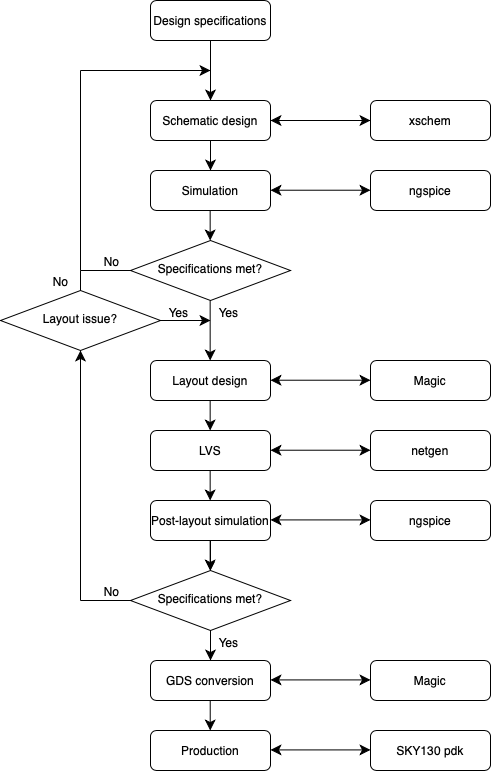
\includegraphics[width=0.8\textwidth]{Figures/Workflow.drawio.png}
    \caption{Analog IC Design Flow Schematic}
    \label{fig:workflow_schematic}
\end{figure}

\section{Design Stages and Their Purpose}

\subsection{Design Concept (Python)}

The initial stage of the design process involves formulating and modeling the idea. This stage leverages mathematical and simulation tools such as Python, along with libraries like NumPy and SciPy, to create preliminary models and validate initial concepts.

\subsection{Schematic Entry (Xschem)}

In this stage, the design specifications are translated into a schematic diagram using tools like Xschem. Xschem is known for its user-friendly interface, which simplifies the process of creating and managing schematic diagrams.

\subsection{Simulation (ngspice)}

Once the schematic is complete, the design is simulated using ngspice. This simulation tool ensures that the design operates correctly within the defined specifications, allowing for the identification and correction of any issues early in the process.

\subsection{Layout (Magic)}

The physical design stage involves drawing the geometries that will form the semiconductor device's layers. Magic is used for this purpose, providing a robust platform for creating the layout while adhering to design rules.

\subsection{Design Rule Check (DRC) (Magic)}

After the layout is complete, Magic provides an interactive design rule check (DRC) to validate that the layout adheres to manufacturing standards. This step is crucial for ensuring that the design can be successfully fabricated.

\subsection{Layout versus Schematic (LVS) (Netgen)}

Netgen is used to compare the layout against the schematic (LVS) to ensure they match perfectly. This verification step is essential to confirm that the physical layout accurately represents the intended circuit design.

\subsection{Device and Parasitic Extraction (Magic)}

Magic also aids in the extraction of parasitic elements that occur during the layout phase. These parasitics can impact the circuit's performance, and their identification allows for further optimization of the design.

\section{Process Design Kits (PDKs)}

Process Design Kits (PDKs) are vital in IC design, providing a collection of manufacturing process-specific rules, tools, and components. For this project, the SkyWater 130nm CMOS sky130 PDK is utilized, offering a comprehensive suite of analog and digital design capabilities.

\section{Documentation of the Design Process in the Wiki}

Throughout this project, extensive documentation was created to aid future designers. The design process, tool presentation, installation steps, and additional resources are thoroughly detailed in the project wiki. This documentation includes:
\begin{itemize}
    \item Detailed instructions on the installation and use of each tool.
    \item Step-by-step guides for each stage of the design process.
    \item Troubleshooting tips and best practices.
    \item Links to further resources and community contributions.
\end{itemize}

For more extensive details on each tool's functions, installation, and integration with the Sky130 PDK, please refer to the wiki pages. This supplementary information is designed to provide a deeper understanding of the toolset used throughout the analog IC design process.

In summary, this workflow chapter provides a comprehensive overview of the stages involved in analog IC design using open-source tools. By following this structured process, we aim to achieve a robust and functional CMOS inverter-based amplifier design.
